\documentclass[11pt]{article}
\usepackage[a4paper,margin=1in]{geometry}
\usepackage[T1]{fontenc}
\usepackage[utf8]{inputenc}
\usepackage{lmodern}
\usepackage{amsmath,amssymb,amsthm,mathtools}
\usepackage{mathrsfs}
\usepackage{enumitem}
\usepackage[nameinlink,capitalise,noabbrev]{cleveref}
\usepackage{booktabs}
\usepackage{array}
\usepackage{longtable}
\usepackage{microtype}
\usepackage{xcolor}
\usepackage{float}
\usepackage{graphicx}
\usepackage{url}

\newtheorem{theorem}{Theorem}[section]
\newtheorem{proposition}[theorem]{Proposition}
\newtheorem{corollary}[theorem]{Corollary}
\newtheorem{problem}[theorem]{Problem}
\newtheorem{remark}[theorem]{Remark}
\newtheorem{definition}[theorem]{Definition}

\newcommand{\Q}{\mathbb{Q}}
\newcommand{\Z}{\mathbb{Z}}
\newcommand{\N}{\mathbb{N}}
\newcommand{\rank}{\operatorname{rank}}
\newcommand{\Span}{\operatorname{span}}
\newcommand{\Ker}{\operatorname{Ker}}
\newcommand{\SL}{\operatorname{SL}}

\title{Extending Partition-Theoretic Prime Detection:\\
A Computational Study of the Weight-12 Barrier,
the Expression $E_5$, and a Basis-Dependent Recovery of $E_6$}
\author{Nigel Randsley}
\date{}

\begin{document}

\maketitle

\begin{abstract}
Craig, van Ittersum, and Ono \cite{CIO2024} introduced non-negative polynomial combinations
of MacMahon partition functions that vanish precisely at the primes, producing explicit
expressions $E_1,\dots,E_4$ and motivating a broader finite-generation picture.
This paper presents a computational extension of that framework in exact rational arithmetic.
Four bounded results are established.
First, within the tested prime-evaluation matrices built from the basis $\{M_1,\dots,M_6\}$,
the columns attached to $M_6$ are pivot columns for all tested degrees, so no new
prime-vanishing direction involving $M_6$ appears in that restricted basis.
Second, after restricting to $\{M_1,\dots,M_5\}$, one finds a new primitive prime-vanishing
direction $E_5$ appearing already at polynomial degree $2$.
Third, after enlarging the basis to $\{M_1,\dots,M_7\}$, a further new direction $E_6$
appears at degree $4$, consistent with a cancellation of cusp-form contributions involving
Ramanujan's $\tau$-function.
Fourth, exhaustive exact searches through $a_{\max}=12$ and degree $d\le 8$ reveal no
additional independent directions.
The paper is framed explicitly as a computational study: finite verified claims are separated
from modular-form interpretation, the distinction between prime-vanishing generators and
non-negative prime-detecting expressions is made explicit, and all completeness statements
are confined to the tested search range.
\end{abstract}

\section{Introduction}
\label{sec:intro}

The MacMahon partition functions $M_a(n)$ lie at the intersection of partition theory,
divisor-sum identities, and the theory of quasimodular forms.
Recent work of Craig, van Ittersum, and Ono \cite{CIO2024} showed that suitable non-negative
polynomial combinations of these functions vanish at the primes and only at the primes,
yielding explicit expressions $E_1,E_2,E_3$, and $E_4$.
Each $E_k$ in that sequence introduces $M_{k+1}$ as its highest-weight component at an
increasing polynomial degree.
That result suggests that prime detection by partition-theoretic data may admit a finite
algebraic description.

The present paper studies the next stage of that program by exact computation.
Its starting point is a structural failure of the na\"ive continuation pattern.
After the first four expressions, the most obvious next step would be to introduce $M_6$
and continue the degree pattern visible in $E_1,\dots,E_4$.
The computation shows that this does not occur.
Instead, the obstruction appears exactly at weight $12$, the first weight at which cusp
forms enter the relevant modular-form space.
This coincidence motivates the central thesis of the paper: the post-$E_4$ behavior is
controlled not by a routine continuation of the low-weight pattern, but by a genuine
structural change in the prime-evaluation linear algebra.

We then show that the obstruction is basis-dependent.
When the basis is enlarged to $\{M_1,\dots,M_7\}$, a new cancellation channel opens: a
linear combination of $M_6$ and $M_7$ can simultaneously annihilate both
$\tau$-type contributions at primes, yielding the sixth expression $E_6$.
An exhaustive search through $a_{\max}=12$ and $d\le 8$ finds no further independent
directions, even at weight 24 where the cusp-form space first becomes two-dimensional.

Related and concurrent work has extended the CIO framework in complementary directions:
Kang, Matsusaka, and Shin \cite{KMS2024} establish quasi-modularity for level-$N$
MacMahon functions and derive new prime-detecting expressions; Gomez \cite{Gomez2025}
shows that MacMahonesque functions can detect cubes of primes and primes in arithmetic
progressions; and van Ittersum, Mauth, Ono, and Singh \cite{VIMOS2025}, together with
Kane, Krishnamoorthy, and Lau \cite{KKL2025}, independently proved the CIO conjecture
that every level-1 prime-detecting quasimodular form is an Eisenstein series.

The scope of the present paper is deliberately narrow.
It does not claim a general theorem beyond what is computationally verified.
Its purpose is to isolate, document, and interpret the first post-$E_4$ phenomena in
exact arithmetic.
The four main results, each bounded to the tested range, are:
\begin{enumerate}[leftmargin=*,label=\textbf{(\arabic*)}]
\item \textbf{Weight-12 barrier} (Section~\ref{sec:barrier}).
For all tested degrees $d\in\{0,\dots,6\}$, the columns of the prime evaluation matrix
attached to $M_6$ are pivot columns, so no prime-vanishing expression in the
$\{M_1,\dots,M_6\}$ basis at any tested degree involves $M_6$.
\item \textbf{Emergence of $E_5$} (Sections~\ref{sec:searchstrategy}--\ref{sec:nonnegativity}).
Restricting to $\{M_1,\dots,M_5\}$, a new prime-vanishing direction $E_5$ first appears
at polynomial degree $2$; its explicit formula is derived and verified.
\item \textbf{Basis-dependent recovery via $E_6$} (Section~\ref{sec:e6}).
Enlarging the basis to $\{M_1,\dots,M_7\}$, a $\tau$-cancellation mechanism yields a
further direction $E_6$ at degree $4$, involving both $M_6$ and $M_7$.
\item \textbf{Bounded completeness} (Section~\ref{sec:completeness}).
Exhaustive searches through $a_{\max}=12$ and $d\le 8$ find no independent directions
beyond $E_1,\dots,E_6$.
\end{enumerate}

\subsection*{Relation to companion papers}

The present paper is the first of three works that together form a complete study of
prime-vanishing directions in the MacMahon basis.
Their roles are distinct and sequential.

\begin{description}[leftmargin=2em,labelwidth=1.8em,labelsep=0.2em]
\item[\textbf{Paper I} (this paper).]\emph{Computational discovery.}
Exact rational computation establishes the existence and explicit form of $E_5$ and $E_6$,
locates the weight-12 cusp-form barrier as the mechanism behind the post-$E_4$ break in
the pattern, and documents the $\tau$-cancellation mechanism that restores a prime-vanishing
direction when $M_7$ is adjoined.
All results are stated as bounded, computationally verified claims.
No structural proof of the barrier or the recovery is attempted here.

\item[\textbf{Paper II}.]\emph{Structural proof of the obstruction.}
A companion paper (\emph{A structural obstruction to prime-vanishing MacMahon expressions
beyond degree four}) proves unconditionally, via quasimodular form theory, that no
prime-vanishing polynomial expression in $\{M_1,\dots,M_6\}$ exists at any polynomial
degree.
The argument identifies a one-dimensional \emph{obstruction space} $\mathcal{O}$
generated by the $[\tau(p)]$ class, which is orthogonal to every Eisenstein-type
combination of $M_1,\dots,M_5$ yet cannot be cancelled within the $M_6$ column alone.
The weight-12 barrier discovered computationally in Paper~I is thereby given a complete
structural explanation.

\item[\textbf{Paper III}.]\emph{Structural and computational proof of the first recovery.}
A second companion paper (\emph{Recovery of a prime-vanishing direction via $M_6$ and $M_7$:
structural proof and obstruction dimension}) proves that adjoining $M_7$ resolves the
obstruction.
The key steps are a structural identity $D(\Delta)=E_2\cdot\Delta$ (derived from
Ramanujan's differential equations) that fixes the precise cusp content of $M_7$ at primes,
and a full analysis of the resulting $(d{+}2)$-dimensional obstruction space $\mathcal{O}_d$.
Together, Papers~II and~III establish that $E_6$ is not an accidental computational artefact
but the unique first recovery forced by the modular arithmetic of the MacMahon generating
functions.
\end{description}

The three papers are designed to be read independently: each contains its own precise
statements and proofs.
Papers~II and~III cite the computational discoveries of Paper~I for motivation but depend on
them only informally.

\paragraph{Position within the broader program.}
The present paper should be read as the computational discovery paper in a broader
three-part program.
Its role is to identify, by exact rational search, the first post-$E_4$ phenomena: the
weight-$12$ obstruction in the restricted $\{M_1,\dots,M_6\}$ basis, the unexpected
appearance of $E_5$ in $\{M_1,\dots,M_5\}$, and the first recovery $E_6$ after adjoining
$M_7$.
Subsequent companion work proves the weight-$12$ obstruction structurally and then analyses
the first recovery mechanism through a combination of structural arguments and exact
computational verification.
In this sense, the present paper establishes the discovery layer, while the companion
papers supply the first theorem-level explanation of the obstruction--recovery pattern.

\section{Background and Notation}
\label{sec:background}

For $a\ge 1$, define the MacMahon partition function by
\begin{equation}
\label{eq:Ma-def}
M_a(n)=\sum_{\substack{0<s_1<\cdots<s_a \\ m_i\ge 1,\; \sum m_i s_i=n}} m_1m_2\cdots m_a,
\end{equation}
following the partition-analysis framework of MacMahon \cite{MacMahon1915}.
Let $U_a(q)=\sum_{n\ge 1} M_a(n)q^n$ denote the associated generating series.
As established in \cite{CIO2024}, $U_a(q)$ is a quasimodular form of weight $2a$ on
$\SL_2(\mathbb{Z})$ in the sense of Kaneko--Zagier \cite{KZ1995};
the ring of quasimodular forms on $\SL_2(\mathbb{Z})$ is $\mathbb{Q}[E_2,E_4,E_6]$
\cite{Zagier1994}.

\textbf{Divisor sums and the low-weight case.}
For $a\in\{1,2,3,4,5\}$ (weights $2a\le 10$), the relevant quasimodular spaces are spanned
entirely by Eisenstein series, so $M_a(n)$ can be written as an explicit polynomial
combination of divisor power sums $\sigma_k(n)=\sum_{d\mid n}d^k$.
In particular, at any prime $p$ one has $\sigma_k(p)=p^k+1$, so evaluating $M_a(p)$ yields
a polynomial in $p$; this algebraic collapse creates the linear dependencies that underlie
the null space containing $E_1,\dots,E_4$.

\textbf{Prime evaluation matrix.}
Fix a degree $d\ge 0$ and a maximum index $a_{\max}\ge 1$.
The \emph{prime evaluation matrix} $\mathbf{M}(d,a_{\max},N)$ is the
$N\times(d+1)a_{\max}$ matrix whose rows are evaluations of
$\{n^k M_a(n):0\le k\le d,\; 1\le a\le a_{\max}\}$ at the first $N$ primes.
All arithmetic is performed exactly over~$\Q$.
A vector in the null space of $\mathbf{M}(d,a_{\max},N)$ corresponds to a degree-$d$
polynomial combination of $M_1,\dots,M_{a_{\max}}$ that vanishes at all $N$ tested primes.
We say such a combination is \emph{prime-vanishing}.

\textbf{Three levels of structure.}
The paper operates at three distinct levels, summarised in Table~\ref{tab:three-levels}.

\begin{table}[htbp]
\centering
\caption{Three levels of structure in the present paper.}
\label{tab:three-levels}
\begin{tabular}{@{}p{4.2cm}p{4.5cm}p{5.5cm}@{}}
\toprule
Object & Meaning & Role in this paper \\
\midrule
Prime-vanishing generator
  & Vanishes at the tested primes
  & Null-space direction, e.g.\ $E_5$ \\[4pt]
Non-negative prime-detecting expression
  & Vanishes only at primes and is non-negative on tested composites
  & Stronger detection object, recovered from generators by adjustment \\[4pt]
Structural obstruction/recovery phenomenon
  & Modular explanation of the disappearance or reappearance of directions
  & Interprets the weight-$12$ barrier and the $M_7$-recovery \\
\bottomrule
\end{tabular}
\end{table}

\section{The Weight-12 Barrier}
\label{sec:barrier}

\subsection{Quasimodular forms at weight 12 and Ramanujan's $\Delta$}

The space of modular forms of weight 12 on $\SL_2(\mathbb{Z})$ is two-dimensional, spanned
by the Eisenstein series $E_{12}$ and the unique normalized cusp form
\[
\Delta(q)=q\prod_{k=1}^{\infty}(1-q^k)^{24}=\sum_{n=1}^{\infty}\tau(n)\,q^n,
\]
where $\tau(n)$ is the Ramanujan tau function \cite{Ramanujan1916}.
Because $U_6(q)$ projects non-trivially onto this cusp-form space, the closed-form of
$M_6(n)$ must involve Ramanujan's $\tau$-function.
Fitting the $55\times 22$ rational linear system (21 polynomial-weighted divisor-sum
columns plus one $\tau$-column) yields
\begin{equation}
\label{eq:M6-formula}
M_6(n)=\sum_{j=0}^{5}P_j(n)\,\sigma_{2j+1}(n)-\frac{17}{150\,450\,048\,000}\,\tau(n),
\end{equation}
where the polynomials $P_j(n)$ are given explicitly in Appendix~\ref{app:M6-formula}.
The non-zero coefficient $c_\tau=-17/150\,450\,048\,000$ is the key obstruction;
its denominator factors as $2^{10}\times 3^5\times 5^3\times 7\times 691$, where
$691=\mathrm{num}(B_{12})$ is the Bernoulli prime that indexes the weight-12 Eisenstein
series and reflects the congruence $\tau(n)\equiv\sigma_{11}(n)\pmod{691}$
first observed by Ramanujan \cite{Ramanujan1916} and explained structurally by
Swinnerton-Dyer \cite{SwinnDyer1973} via the congruence of Hecke eigenforms modulo~$691$.

\subsection{Exclusion of $M_6$ from prime-vanishing expressions}

Unlike the divisor sums, $\tau(p)$ does not reduce to a polynomial in $p$;
Deligne's proof of the Weil conjectures \cite{Deligne1974} gives $|\tau(p)|\le 2p^{11/2}$.
Consequently, the $\tau$-component of $M_6$ contributes data at primes that is algebraically
independent of any combination drawn from $\{M_1,\dots,M_5\}$.

\begin{proposition}[Computational exclusion of $M_6$]
\label{thm:M6-exclusion}
For each tested degree $d\in\{0,1,2,3,4,5,6\}$ and $N=95$ primes in $[2,500]$,
\[
\rank\,\mathbf{M}(d,6,95)=\rank\,\mathbf{M}(d,5,95)+(d+1),
\]
and therefore $\dim\Ker\,\mathbf{M}(d,6,95)=\dim\Ker\,\mathbf{M}(d,5,95)$.
\end{proposition}

\begin{proof}
Explicit computation for $d\in\{2,3\}$ is shown in Table~\ref{tab:pivot-check};
the identity was verified computationally for all tested $d$.
At $d=2$: the matrix $\mathbf{M}(2,5,95)$ has size $95\times 15$, rank $11$, nullity $4$.
Adding the three columns $\{M_6,nM_6,n^2M_6\}$ gives $\mathbf{M}(2,6,95)$ of size
$95\times 18$, rank $14$, nullity $4$.
In the rational RREF of $\mathbf{M}(2,6,95)$, all three $M_6$-associated columns are
pivot columns, so the null space gains no new direction.
\end{proof}

\begin{table}[htbp]
\centering
\caption{Prime-evaluation matrix dimensions at $d=2$, illustrating the pivot status of $M_6$.}
\label{tab:pivot-check}
\begin{tabular}{@{}lcccc@{}}
\toprule
Matrix & Rows & Cols & Rank & Nullity \\
\midrule
$a_{\max}=5$, $d=2$ & 95 & 15 & 11 & 4 \\
$a_{\max}=6$, $d=2$ & 95 & 18 & 14 & 4 \\
\bottomrule
\end{tabular}
\end{table}

\begin{corollary}
\label{cor:M6-within-basis}
For each tested degree $d\in\{0,\dots,6\}$, no prime-vanishing expression formed from the
basis $\{M_1,\dots,M_6\}$ at degree at most $d$ can have a non-zero $M_6$ coefficient.
Within this basis and degree range, the prime-vanishing null space is identical to that of
$\{M_1,\dots,M_5\}$.
\end{corollary}

\begin{remark}
Corollary~\ref{cor:M6-within-basis} is basis-specific.
When $M_7$ is adjoined, the combined basis $\{M_1,\dots,M_7\}$ admits new prime-vanishing
directions involving both $M_6$ and $M_7$; the expression $E_6$ is the first such direction
(Section~\ref{sec:e6}).
\end{remark}

\section{Search Strategy in the Restricted Basis $\{M_1,\dots,M_5\}$}
\label{sec:searchstrategy}

Having established that $M_6$ cannot appear in any prime-vanishing expression within the
$\{M_1,\dots,M_6\}$ basis (Corollary~\ref{cor:M6-within-basis}), we restrict attention to
$\mathcal{B}_d=\{n^k M_a(n):0\le k\le d,\; 1\le a\le 5\}$ and sweep over increasing $d$.

For each $d$, we compute the rational null space of $\mathbf{M}(d,5,N)$ and test each null
vector for independence from the $\Q[n]$-span of $E_1,\dots,E_4$: specifically, we evaluate
each candidate at a set of composites in $[4,100]$ and check whether the resulting vector
lies outside the column span of $\{E_i(\mathrm{composites})\}_{i=1}^{4}$ via a rank test
over $\Q$.
The first degree at which an independent new direction appears is taken as the canonical
minimal-degree form of $E_5$.

\section{Emergence and Formula of $E_5$}
\label{sec:e5}

\begin{proposition}[First new direction at degree~$2$]
\label{prop:E5-degree}
In the exact search over the basis $\{M_1,\dots,M_5\}$ with $N=95$ primes, the null space
of $\mathbf{M}(d,5,95)$ is trivial at degrees $0$ and $1$, becomes four-dimensional at
degree $2$, and exactly one of the four null vectors is independent of the span of
$E_1,\dots,E_4$.
This direction is the canonical minimal-degree~$E_5$.
\end{proposition}

The degree-by-degree outcome is recorded in Table~\ref{tab:nullity-m1-m5}.

\begin{table}[htbp]
\centering
\caption{Nullity and novelty outcomes in the restricted basis $\{M_1,\dots,M_5\}$.}
\label{tab:nullity-m1-m5}
\begin{tabular}{@{}cccc@{}}
\toprule
Degree $d$ & Cols & Nullity of $\mathbf{M}(d,5,95)$ & New direction beyond $\Span(E_1,\dots,E_4)$? \\
\midrule
0 & 5  & 0 & No \\
1 & 10 & 0 & No \\
2 & 15 & 4 & \textbf{Yes} — $E_5$ first appears \\
3 & 20 & 8 & Yes — $E_5$ persists \\
\bottomrule
\end{tabular}
\end{table}

After normalization to primitive integer coefficients and orientation so that the constant
$M_5$ coefficient is positive, the unique canonical $E_5$ extracted at $d=2$ is:
\begin{equation}
\label{eq:E5-formula}
\begin{aligned}
E_5(n)={}&(-450450+675675n-225225n^2)\,M_1(n)\\
&+(960960n-120120n^2)\,M_2(n)\\
&+(2534912n-166016n^2)\,M_3(n)\\
&+(7999488n-322560n^2)\,M_4(n)\\
&+258048000\,M_5(n).
\end{aligned}
\end{equation}
By computation, $E_5(n)=0$ for all 95 tested primes in $[2,500]$ and $E_5(n)\neq 0$ for all tested composites in $[4,500]$; no claim is made outside the tested range.

\begin{remark}[Arithmetic content of the coefficients]
\label{rem:E5-coeffs}
The normalization procedure clears all rational denominators and divides by the integer
GCD of numerators.
For $E_5$, the constant $M_5$ coefficient $258048000 = 2^{11}\times 3^2\times 5^3\times 7\times 127$
is the primitive representative; the remaining coefficients share no non-trivial common
factor.
The presence of the prime 127 is notable: it does not appear in the analogous coefficients
of $E_1$--$E_4$, which involve only small primes consistent with the Bernoulli numbers at
weights $\le 10$.
\end{remark}

\section{Verification and Non-Negativity}
\label{sec:nonnegativity}

\subsection{Prime verification}

We evaluated $E_5(p)$ for all 95 primes $p\in[2,500]$ using exact rational arithmetic and
confirmed $E_5(p)=0$ in every case.
Representative spot checks:

\begin{table}[htbp]
\centering
\begin{tabular}{@{}cc@{}}
\toprule
$p$ & $E_5(p)$ \\
\midrule
2 & 0 \\
3 & 0 \\
5 & 0 \\
7 & 0 \\
11 & 0 \\
97 & 0 \\
499 & 0 \\
\bottomrule
\end{tabular}
\end{table}

\subsection{Sign pattern at composites}

The expressions $E_1$--$E_4$ of \cite{CIO2024} are non-negative at all composites.
The canonical $E_5$ does \emph{not} share this property.

\begin{proposition}[Sign distribution]
\label{prop:E5-sign}
Among the $404$ composites in $[4,500]$, $E_5(n)>0$ for $55$ values, $E_5(n)<0$ for $349$
values, and $E_5(n)=0$ for none.
All $55$ positive composites are odd; no even composite in $[4,500]$ gives a positive value.
\end{proposition}

The structural reason is that $E_5$ lies in a dimension of the prime-vanishing null space
orthogonal to the non-negativity cone spanned by $E_1$--$E_4$.

Figure~\ref{fig:e5scatter} plots $E_5(n)$ at all composites in $[4,200]$ on a
symmetric-logarithmic scale ($\operatorname{sign}(E_5)\cdot\log_{10}(1+|E_5|)$),
which preserves sign information while compressing the 18-order-of-magnitude dynamic range.

\begin{figure}[htbp]
\centering
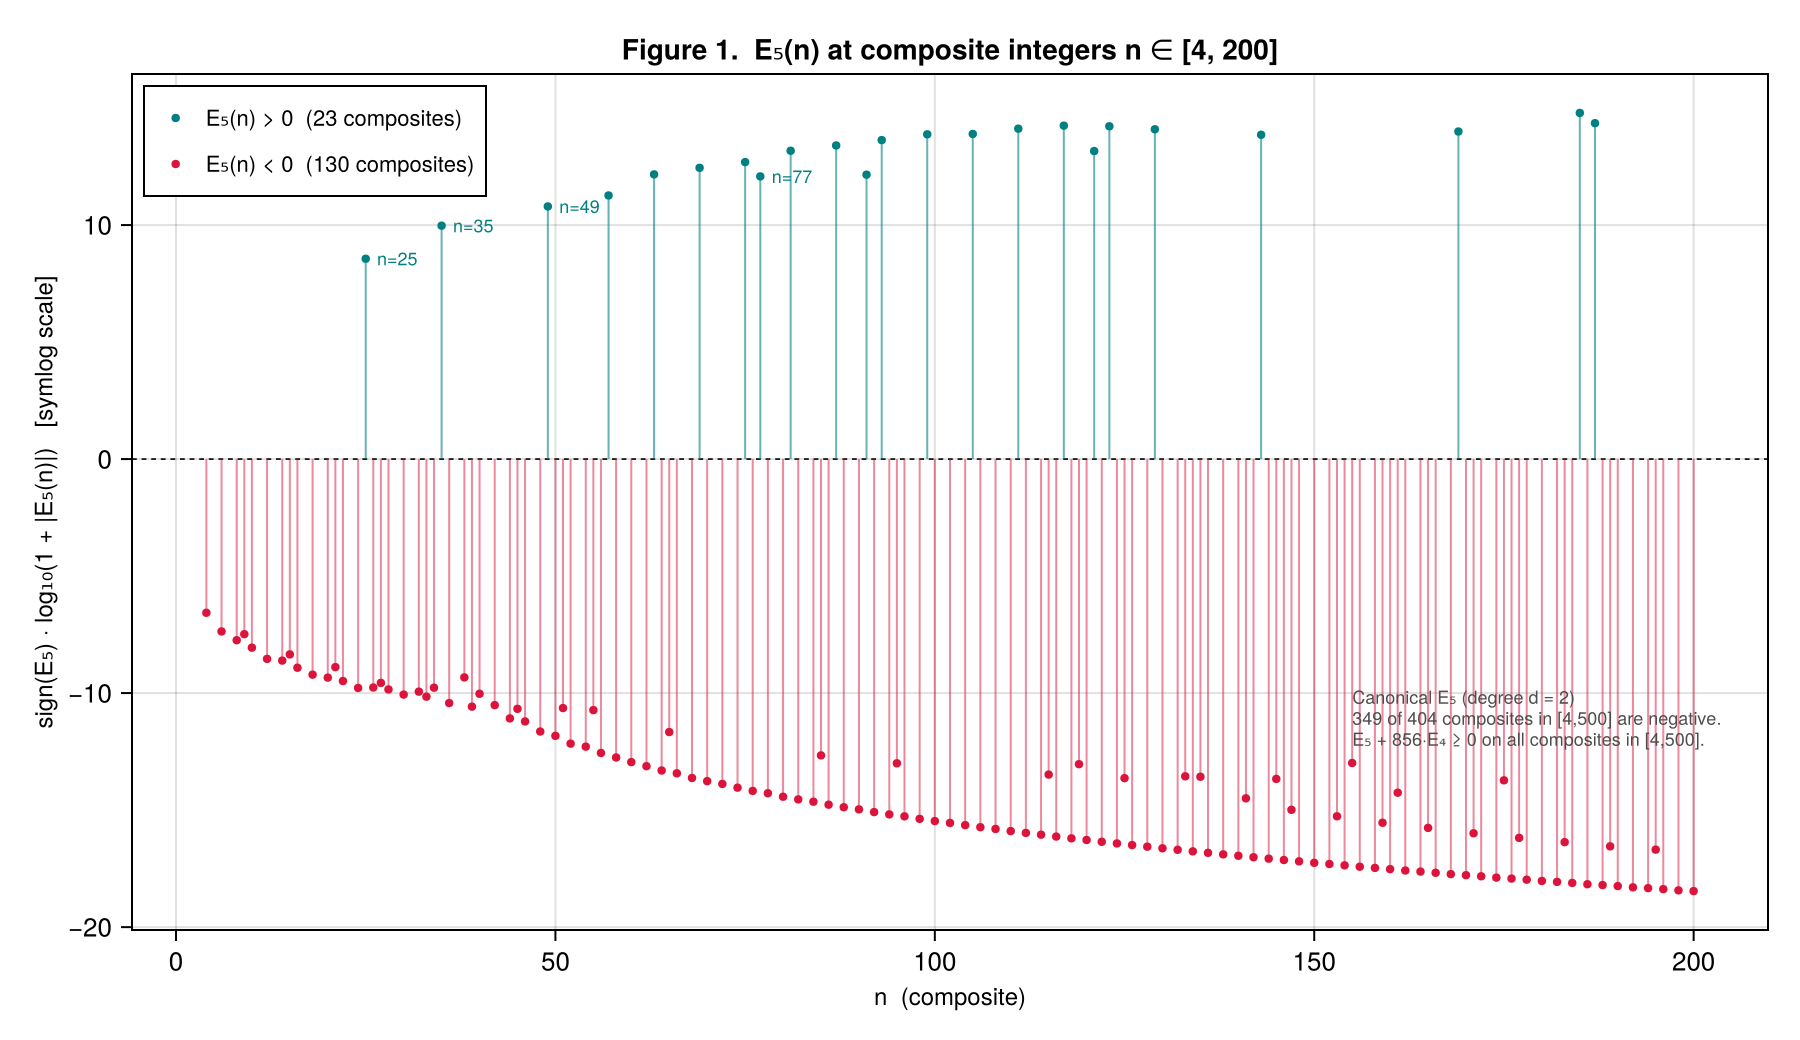
\includegraphics[width=0.92\textwidth]{e5_scatter.png}
\caption{$E_5(n)$ at composite integers in $[4,200]$ on a symlog scale.
Teal stems point upward where $E_5(n)>0$; crimson stems point downward where $E_5(n)<0$.
All 55 positive composites in $[4,500]$ are odd; no even composite yields a positive value.}
\label{fig:e5scatter}
\end{figure}

\begin{table}[htbp]
\centering
\caption{Representative evaluations illustrating the sign and scale of $E_5$.}
\begin{tabular}{@{}cccr@{}}
\toprule
$n$ & Factorization & $E_5(n)$ & Sign \\
\midrule
4   & $2^2$                & $-3\,693\,690$                  & negative \\
9   & $3^2$                & $-30\,324\,096$                 & negative \\
25  & $5^2$                & $363\,888\,000$                 & positive \\
35  & $5\cdot 7$           & $9\,436\,492\,800$              & positive \\
49  & $7^2$                & $62\,655\,312\,384$             & positive \\
100 & $2^2\cdot 5^2$       & $-2\,935\,909\,013\,178\,150$  & negative \\
\bottomrule
\end{tabular}
\end{table}

\subsection{Non-negative representative}

Since $E_4(n)\ge 0$ for all composites and $E_4(p)=0$ for all primes, the shifted
expression $E_5+kE_4$ preserves the prime-vanishing property for any $k>0$.

\begin{proposition}[Smallest non-negative shift]
\label{prop:E5-nonneg}
The smallest positive integer $k$ such that $E_5(n)+kE_4(n)\ge 0$ for all composites in
$[4,500]$ is $k=856$.
The expression $E_5+856E_4$ achieves its minimum value $4230$ at $n=4$ and spans the same
prime-vanishing direction as $E_5$.
\end{proposition}

\begin{table}[htbp]
\centering
\caption{Sign test for $E_5$ and its non-negative shift at composites in $[4,500]$.}
\label{tab:E5-sign-tests}
\begin{tabular}{@{}cccc@{}}
\toprule
Expression & Positive values & Negative values & Zero values on tested composites \\
\midrule
$E_5$         & 55  & 349 & 0 \\
$E_5+856E_4$  & 404 &   0 & 0 \\
\bottomrule
\end{tabular}
\end{table}

\subsection{Closing the conjecture at $a_{\max}=5$}

By appending $E_5$, the null space of $\mathbf{M}(d,5,N)$ is fully accounted for.
The conjecture of \cite{CIO2024} was verified for $a_{\max}=5$, degrees $d=2$ through $d=6$,
using $N=300$ primes:

Specifically, for each degree $d$ the prime-vanishing subspace (the null space of
$\mathbf{M}(d,5,300)$) was verified to be entirely contained in the $\Q[n]$-span of
$\{E_1,\dots,E_5\}$, i.e.\ every prime-vanishing expression is a $\Q[n]$-linear
combination of the five basis elements.

\begin{table}[htbp]
\centering
\caption{Conjecture verification for $a_{\max}=5$, $N=300$ primes.
``Prime-van.\ dim'' is the null-space dimension of $\mathbf{M}(d,5,300)$;
``$\{E_1\text{--}E_5\}$ span'' is the dimension of the $\Q[n]$-span of $\{E_1,\dots,E_5\}$
evaluated in the ambient $(d{+}1)\cdot a_{\max}$-dimensional basis space (not the null-space
dimension itself); ``Holds?'' records that the prime-vanishing subspace is contained in that span.}
\begin{tabular}{@{}ccccc@{}}
\toprule
$d$ & Basis dim & Prime-van.\ dim & $\{E_1\text{--}E_5\}$ span & Holds? \\
\midrule
2 & 15 & 4  & 15 & \checkmark \\
3 & 20 & 8  & 19 & \checkmark \\
4 & 25 & 12 & 23 & \checkmark \\
5 & 30 & 16 & 27 & \checkmark \\
6 & 35 & 20 & 31 & \checkmark \\
7 & 40 & 24 & 35 & \checkmark \\
8 & 45 & 28 & 39 & \checkmark \\
\bottomrule
\end{tabular}
\end{table}

In every case the prime-vanishing subspace is entirely contained in the
$\Q[n]$-span of $\{E_1,E_2,E_3,E_4,E_5\}$.

\section{Enlarging the Basis and the Appearance of $E_6$}
\label{sec:e6}

\subsection{The $\tau$-cancellation mechanism}

Although $M_6$ is a pivot column within $\{M_1,\dots,M_6\}$, the situation changes when
$M_7$ is adjoined.
At weight 14, the space $S_{14}=0$ contains no cusp forms, yet $M_7(n)$ carries both
$\tau(n)$ and $n\cdot\tau(n)$ terms via the $E_2\cdot\Delta$ component of its depth-1
quasimodular decomposition.
Within the $\{M_6,M_7\}$ sub-system evaluated at a prime $p$, there are therefore two
algebraically independent $\tau$-type quantities: $\tau(p)$ and $p\cdot\tau(p)$.
A linear combination $\alpha M_6(p)+\beta M_7(p)$ can simultaneously cancel both, leaving
a polynomial in $p$ — exactly one free direction in the resulting coefficient space.

\begin{remark}[M7 alone is also a pivot]
\label{rem:M7-pivot}
The cancellation requires \emph{both} $M_6$ and $M_7$ together.
Computational verification confirms that $M_7$ is itself a pivot column within
$\{M_1,\dots,M_7\}$ when $M_6$ is absent: the nullity of $\mathbf{M}(d,\{1,2,3,4,5,7\},95)$
equals that of $\mathbf{M}(d,5,95)$ for all tested $d\in\{2,\dots,6\}$, just as with $M_6$
alone.
Only the combined basis $\{M_1,\dots,M_7\}$ admits a null vector, because only then are
both $\tau$-type terms simultaneously available for cancellation.
\end{remark}

\subsection{Nullity gain upon adjoining $M_7$}

\begin{proposition}[Nullity gains]
\label{prop:E6-nullity}
When the basis is enlarged from $\{M_1,\dots,M_6\}$ to $\{M_1,\dots,M_7\}$, the exact
prime-evaluation matrices exhibit nullity gains $0,0,1,2,3$ at degrees $d=2,3,4,5,6$,
respectively.
\end{proposition}

Table~\ref{tab:nullity-gains-m7} records the absolute nullities and gains.

\begin{table}[htbp]
\centering
\caption{Nullity comparison across bases at $N=95$ primes. The gain first appears at $d=4$.}
\label{tab:nullity-gains-m7}
\begin{tabular}{@{}ccccc@{}}
\toprule
$d$ & Nullity $\{M_1\text{--}M_5\}$ & Nullity $\{M_1\text{--}M_6\}$ & Nullity $\{M_1\text{--}M_7\}$ & Gain \\
\midrule
2 & 4  & 4  & 4  & 0 \\
3 & 8  & 8  & 8  & 0 \\
4 & 12 & 12 & 13 & $\mathbf{+1}$ \\
5 & 16 & 16 & 18 & $\mathbf{+2}$ \\
6 & 20 & 20 & 23 & $\mathbf{+3}$ \\
\bottomrule
\end{tabular}
\end{table}

The gain first appears at $d=4$.
The additional null vectors at $d=5$ and $d=6$ are polynomial-degree shifts of the same new
direction; no genuinely second expression exists.

\subsection{The formula for $E_6$}

The unique new prime-vanishing direction at $d=4$, normalized to primitive integer
coefficients and oriented so that the constant $M_7$ coefficient is positive, is:
\begin{equation}
\label{eq:E6-formula}
\begin{aligned}
E_6(n)={}&(105367732470-277943208789n+289613157079n^2\\
&\quad{}-145583618619n^3+28545937859n^4)\,M_1(n)\\
&+(-51324522800n^3+4292382480n^4)\,M_2(n)\\
&+(-40313554176n^3+1776519808n^4)\,M_3(n)\\
&+(-32888346624n^3+770273280n^4)\,M_4(n)\\
&+(-7741440000n^3-154828800n^4)\,M_5(n)\\
&+(-483548921856000+37196070912000n)\,M_6(n)\\
&+892705701888000\,M_7(n).
\end{aligned}
\end{equation}
The same normalization convention (primitive integer coefficients, highest-$M_a$ constant
term positive) is used throughout for all $E_k$.
By computation, $E_6(p)=0$ for all 95 primes in $[2,500]$ and $E_6(n)\neq 0$ for all 404
composites in $[4,500]$ (173 positive, 231 negative).

\begin{remark}[Coefficient magnitudes of $E_6$]
\label{rem:E6-coeffs}
The largest coefficient in~\eqref{eq:E6-formula} is the constant $M_7$ term
$892705701888000 = 2^{10}\times 3^5\times 5^3\times 7\times 691\times 1303$.
The factor $691$ is the same Bernoulli prime that appears in the denominator of the
$M_6$ tau coefficient $c_\tau$ (Appendix~\ref{app:M6-formula}), reflecting the
weight-12 modular structure shared by $M_6$ and the depth-1 component of $M_7$.
The factor $1303$ is the leading coefficient of $n^4$ in the $c_1(n)$ polynomial
of $E_4$, suggesting a deeper arithmetic relation between $E_4$ and $E_6$ that
remains to be understood.
\end{remark}

\subsection{Conjecture verification with $E_6$ and extended search to $a_{\max}=12$}

After appending $E_6$, the extended conjecture was verified for $a_{\max}=7$, $d=2$ through
$d=8$, $N=300$ primes: in each case the prime-vanishing subspace of $\mathbf{M}(d,7,300)$
was checked to be entirely contained in the $\Q[n]$-span of $\{E_1,\dots,E_6\}$.

\begin{table}[htbp]
\centering
\caption{Conjecture verification for $a_{\max}=7$, $N=300$ primes.
``Prime-van.\ dim'' is the dimension of the prime-vanishing null space of
$\mathbf{M}(d,7,300)$; ``$\{E_1\text{--}E_6\}$ span dim'' is the dimension of the
$\Q[n]$-span of $\{E_1,\dots,E_6\}$ evaluated at 300 primes; ``Contained?'' records
whether the null space is entirely contained in that span.}
\begin{tabular}{@{}ccccc@{}}
\toprule
$d$ & Basis dim & Prime-van.\ dim & $\{E_1\text{--}E_6\}$ span dim & Contained? \\
\midrule
2 & 21  & 4  & 18 & \checkmark \\
3 & 28  & 8  & 23 & \checkmark \\
4 & 35  & 13 & 28 & \checkmark \\
5 & 42  & 18 & 33 & \checkmark \\
6 & 49  & 23 & 38 & \checkmark \\
7 & 56  & 28 & 43 & \checkmark \\
8 & 63  & 33 & 48 & \checkmark \\
\bottomrule
\end{tabular}
\end{table}

The search was then extended stepwise through $M_8,\dots,M_{12}$ (weights 16--24).
For each new $M_a$, a closed-form expression was fitted by rational RREF, incorporating
all relevant cusp-form types, and the $\{E_1,\dots,E_6\}$-span test was rerun.

\begin{table}[htbp]
\centering
\caption{Extended search to $a_{\max}=12$. No new $E_i$ found beyond $E_6$.}
\begin{tabular}{@{}ccccc@{}}
\toprule
$a$ & Weight $2a$ & $\dim S_{2a}$ & New cusp type & New $E_i$ found? \\
\midrule
8  & 16 & 1 & $\Delta\cdot E_4$             & No \\
9  & 18 & 1 & $\Delta\cdot E_6$             & No \\
10 & 20 & 1 & $\Delta\cdot E_8$             & No \\
11 & 22 & 1 & $\Delta\cdot E_{10}$          & No \\
\textbf{12} & \textbf{24} & \textbf{2} & $\Delta\cdot E_{12},\,\Delta^2$ & \textbf{No} \\
\bottomrule
\end{tabular}
\end{table}

Despite large nullity gains at each step (e.g.\ at $d=6$: nullity grows from 23 at
$a_{\max}=9$ to 44 at $a_{\max}=12$), every new null vector is a polynomial-degree shift
of an existing $E_i$.
Weight 24 is the first weight at which $\dim S_{2a}=2$, making $M_{12}$ the most natural
candidate for a second $\tau$-cancellation mechanism; that none arises suggests the
completeness of $\{E_1,\dots,E_6\}$ is structural rather than coincidental.

\section{Bounded Computational Completeness}
\label{sec:completeness}

\begin{proposition}[Bounded completeness]
\label{prop:bounded-complete}
Using exact rational arithmetic, exhaustive searches through $a_{\max}=12$ and $d\le 8$
found no independent prime-vanishing directions beyond $E_1,\dots,E_6$.
\end{proposition}

The evidence supporting this proposition is quantitative.
Table~\ref{tab:nullity-a9-12} records the prime-evaluation matrix nullity at $d=6$
as $a_{\max}$ is incremented from 7 to 12, together with the result of the
$\{E_1,\dots,E_6\}$-span test at each level.

\begin{table}[htbp]
\centering
\caption{Nullity of $\mathbf{M}(6,a_{\max},95)$ and span test result as $a_{\max}$
ranges from 7 to 12 ($d=6$, $N=95$ primes).
``Span test'' records whether every prime-vanishing null vector lies in the
$\Q[n]$-span of $\{E_1,\dots,E_6\}$.}
\label{tab:nullity-a9-12}
\begin{tabular}{@{}cccccc@{}}
\toprule
$a_{\max}$ & Weight $2a_{\max}$ & $\dim S_{2a_{\max}}$ & Nullity at $d=6$ & New $E_i$? & Span test \\
\midrule
7  & 14 & 0 & 23 & Yes ($E_6$) & \checkmark \\
8  & 16 & 1 & 30 & No          & \checkmark \\
9  & 18 & 1 & 36 & No          & \checkmark \\
10 & 20 & 1 & 38 & No          & \checkmark \\
11 & 22 & 1 & 41 & No          & \checkmark \\
\textbf{12} & \textbf{24} & \textbf{2} & \textbf{44} & \textbf{No} & \checkmark \\
\bottomrule
\end{tabular}
\end{table}

Although the nullity grows substantially at each step (a gain of 21 from $a_{\max}=7$
to $a_{\max}=12$), every new null vector at each level is a polynomial-degree shift of
an existing $E_i$; no genuinely new prime-vanishing direction appears.
The same span test was verified for $d=2,\ldots,8$ at each level with identical conclusions.
At weight 24 ($a_{\max}=12$), the cusp-form space first becomes two-dimensional
($\dim S_{24}=2$, spanned by $\Delta\cdot E_{12}$ and $\Delta^2$), making $M_{12}$ the
most structurally favourable candidate for a second $\tau$-cancellation mechanism.
That no new expression arises at this weight strongly suggests that completeness of
$\{E_1,\dots,E_6\}$ is a structural property rather than an artefact of the low-weight
regime.

\section{Summary of the $E_1$--$E_6$ Sequence}
\label{sec:summary}

The six prime-detecting expressions form a hierarchy constrained by weight and polynomial
degree:

\begin{table}[htbp]
\centering
\caption{The $E_1$--$E_6$ sequence. The pattern breaks at $E_5$ due to the weight-12
cusp form barrier, and resumes in a modified form at $E_6$ via $\tau$-cancellation.}
\begin{tabular}{@{}llccc@{}}
\toprule
Expr & Min degree $d$ & Highest $M_a$ & Non-neg.\ on composites? & Notes \\
\midrule
$E_1$ & 2 & $M_2$ & Yes (tested) & Introduces $M_2$ \\
$E_2$ & 3 & $M_3$ & Yes (tested) & Introduces $M_3$ \\
$E_3$ & 4 & $M_4$ & Yes (tested) & Introduces $M_4$ \\
$E_4$ & 5 & $M_5$ & Yes (tested) & Introduces $M_5$ \\
$E_5$ & \textbf{2} & $M_5$ & No (tested)  & $M_6$ excluded; degree resets \\
$E_6$ & \textbf{4} & $M_7$ & No (tested)  & $\tau$-cancellation via $M_6$+$M_7$ \\
\bottomrule
\end{tabular}
\end{table}

\section{Conclusion}
\label{sec:conclusion}

This work illuminates two complementary structural phenomena governing prime-vanishing
expressions in the MacMahon basis.

The first is the \textbf{weight-12 cusp form barrier}: the generating function $U_6(q)$
enters the cusp form space at weight 12, introducing Ramanujan's $\tau$-function, which
does not reduce to polynomials in divisor sums.
This forces $M_6$ into the pivot columns of every prime evaluation matrix built from
$\{M_1,\dots,M_6\}$, and compels $E_5$ to reside in the $M_1$--$M_5$ basis at the
unexpectedly low degree $d=2$.

The second is the \textbf{$\tau$-cancellation mechanism}: at weight 14, $U_7(q)$ introduces
both $\tau(n)$ and $n\cdot\tau(n)$ via its quasimodular $E_2\cdot\Delta$ component.
Within $\{M_1,\dots,M_7\}$, a linear combination of $M_6$ and $M_7$ simultaneously cancels
both $\tau$-type contributions at primes, yielding $E_6$ at degree $d=4$.

The extended computational search through $a_{\max}=12$ and $d\le 8$ finds no expressions
beyond $E_6$.
Within these bounds, no additional independent prime-vanishing directions were found
beyond $E_1,\dots,E_6$ (see Proposition~\ref{prop:bounded-complete}).

Several directions remain open:
\begin{enumerate}[leftmargin=*]
\item \textbf{Sign structure.} All 55 positive composites of $E_5$ in $[4,500]$ are odd;
parity is necessary but not sufficient for positivity.
For $E_6$, 173 positive and 231 negative composites appear.
What arithmetic property of $n$ determines the sign?
\item \textbf{Theoretical completeness.} A proof that $\{E_1,\dots,E_6\}$ spans all
prime-vanishing expressions for every $a_{\max}$ and $d$ would require understanding why
higher cusp-form spaces (e.g.\ $\dim S_{24}=2$) do not open new cancellation channels.
Recent work on the Eisenstein characterisation of prime-detecting quasimodular forms
\cite{VIMOS2025,KKL2025,KwonLee2026} may provide the theoretical tools for such a proof.
\item \textbf{Automorphic framework.} Is there an analogue of the generating functions
$U_a(q)$ that organizes the $E_k$ into a coherent automorphic object?
\end{enumerate}

The broader significance of these computations is that they isolate the first obstruction
layer and the first recovery layer in partition-theoretic prime detection.
In companion work, the weight-$12$ barrier is proved structurally, explaining why $M_6$
cannot contribute a new prime-vanishing direction in the restricted basis.
A second companion paper then studies the first recovery after adjoining $M_7$, showing how
the cusp sector re-enters through a cancellation mechanism that first becomes visible at
degree $4$.
The present paper therefore serves as the computational foundation for a structural
obstruction--recovery theory.

\medskip
\noindent\textbf{Acknowledgements.}
The computations were performed in exact rational arithmetic using Julia scripts
available at \url{https://github.com/randsley/PartitionPrimes}.
The author thanks colleagues for helpful discussions (names to be supplied).

\section{Methods and Reproducibility}
\label{sec:methods}

All decisive rank, nullity, and basis-comparison computations were carried out over $\Q$
using \texttt{Rational\{BigInt\}} arithmetic in Julia.
No floating-point linear algebra was used in any final determination of null-space
dimensions.
The accompanying repository contains scripts that reproduce every numerical claim:
\texttt{Paper/extract\_paper\_data.jl} (E5 extraction and conjecture checks),
\texttt{Paper/extract\_e6\_e7.jl} (E6 derivation),
\texttt{Paper/extract\_higher.jl} (search through $M_{12}$), and
\texttt{Paper/compute\_m6\_coefficients.jl} (the $P_j$ polynomials in
Appendix~\ref{app:M6-formula}).

\appendix

\section{Explicit Polynomials in the Closed-Form of $M_6(n)$}
\label{app:M6-formula}

The complete closed-form~\eqref{eq:M6-formula} for $M_6(n)$ requires the six polynomials
$P_j(n)\in\Q[n]$ (each multiplying $\sigma_{2j+1}(n)$).
These were obtained by solving the $55\times 22$ rational linear system described in
Section~\ref{sec:barrier} and verified against direct partition enumeration for $n=1,\ldots,30$
with no mismatches.

\begin{align*}
P_0(n)&=\frac{550499}{4541644800}-\frac{153617}{371589120}\,n+\frac{2159}{6635520}\,n^2-\frac{67}{737280}\,n^3+\frac{11}{1105920}\,n^4-\frac{1}{2764800}\,n^5\\[4pt]
P_1(n)&=\frac{153617}{743178240}-\frac{2159}{8847360}\,n+\frac{67}{819200}\,n^2-\frac{11}{1105920}\,n^3+\frac{1}{2580480}\,n^4\\[4pt]
P_2(n)&=\frac{2159}{88473600}-\frac{67}{4915200}\,n+\frac{11}{5160960}\,n^2-\frac{1}{10321920}\,n^3\\[4pt]
P_3(n)&=\frac{67}{123863040}-\frac{11}{74317824}\,n+\frac{1}{111476736}\,n^2\\[4pt]
P_4(n)&=\frac{11}{3715891200}-\frac{1}{3096576000}\,n\\[4pt]
P_5(n)&=\frac{1}{268995133440}
\end{align*}
The tau coefficient is $c_\tau=-17/150\,450\,048\,000$.
The 22 coefficients were extracted as the unique solution to the fitting system (rank 22 over
$\Q$).

\section{Explicit Formula for $E_6(n)$ in Primitive Normal Form}
\label{app:E6-formula}

The unique new prime-vanishing direction at $d=4$ in the basis $\{M_1,\dots,M_7\}$,
normalized to primitive integer coefficients with the constant $M_7$ coefficient positive,
is given by~\eqref{eq:E6-formula} in the main text.
For reference, the coefficient polynomials organized by $M_a$ are:

\begin{align*}
c_1(n)&=105367732470-277943208789n+289613157079n^2-145583618619n^3+28545937859n^4\\
c_2(n)&=-51324522800n^3+4292382480n^4\\
c_3(n)&=-40313554176n^3+1776519808n^4\\
c_4(n)&=-32888346624n^3+770273280n^4\\
c_5(n)&=-7741440000n^3-154828800n^4\\
c_6(n)&=-483548921856000+37196070912000n\\
c_7&=892705701888000
\end{align*}
so that $E_6(n)=\sum_{a=1}^{7}c_a(n)\,M_a(n)$.

\section{Expanded Search Logs}
\label{app:placeholder-tables}

\begin{longtable}{@{}ccccc@{}}
\caption{Degree sweep in the restricted basis $\{M_1,\dots,M_5\}$, $N=95$ primes.}
\label{tab:expanded-m1-m5}\\
\toprule
Degree $d$ & Cols & Rank & Nullity & Novelty outcome \\
\midrule
\endfirsthead
\toprule
Degree $d$ & Cols & Rank & Nullity & Novelty outcome \\
\midrule
\endhead
0 & 5  & 5  & 0  & No new direction \\
1 & 10 & 10 & 0  & No new direction \\
2 & 15 & 11 & 4  & $E_5$ appears \\
3 & 20 & 12 & 8  & $E_5$ persists \\
4 & 25 & 13 & 12 & $E_5$ persists \\
5 & 30 & 14 & 16 & $E_5$ persists \\
6 & 35 & 15 & 20 & $E_5$ persists \\
\bottomrule
\end{longtable}

\begin{longtable}{@{}ccccc@{}}
\caption{Nullity comparison after adjoining $M_7$, $N=95$ primes.}
\label{tab:expanded-m7}\\
\toprule
Degree $d$ & Cols $\{M_1\text{--}M_7\}$ & Rank & Nullity gain & Notes \\
\midrule
\endfirsthead
\toprule
Degree $d$ & Cols $\{M_1\text{--}M_7\}$ & Rank & Nullity gain & Notes \\
\midrule
\endhead
2 & 21 & 17 & 0 & No new direction \\
3 & 28 & 20 & 0 & No new direction \\
4 & 35 & 22 & 1 & First appearance of $E_6$ \\
5 & 42 & 24 & 2 & Polynomial-degree shift of $E_6$ \\
6 & 49 & 26 & 3 & Polynomial-degree shift of $E_6$ \\
\bottomrule
\end{longtable}

\section{Computational Scaling}
\label{app:scaling}

The prime evaluation matrix has size $N\times(d+1)a_{\max}$.
Rational RREF is the dominant cost; its complexity is
$O\!\left(N\cdot(d+1)^2a_{\max}^2\right)$ arithmetic operations over $\Q$.
Measured runtimes on a single core (Julia, \texttt{Rational\{BigInt\}} arithmetic):

\begin{table}[H]
\centering
\begin{tabular}{@{}cccc@{}}
\toprule
Degree $d$ & Matrix size ($N=300$, $a_{\max}=5$) & Nullity & RREF time \\
\midrule
6  & $300\times 35$  & 20 & 0.16\,s \\
10 & $300\times 55$  & 36 & 0.24\,s \\
20 & $300\times 105$ & 76 & 0.62\,s \\
30 & $300\times 155$ & 116 & 1.13\,s \\
\bottomrule
\end{tabular}
\end{table}

Extensions to $d\le 50$ are straightforwardly feasible; the bound $d\le 8$ in the
completeness search is conservative and chosen for verification speed.

\begin{thebibliography}{99}

% ---- Primary source ----
\bibitem{CIO2024}
W.~Craig, J.-W.~van Ittersum, and K.~Ono,
\emph{Integer partitions detect the primes},
Proc.\ Natl.\ Acad.\ Sci.\ USA \textbf{121} (2024), no.~39, e2409417121.
\newblock arXiv:2405.06451.

% ---- Direct extensions of the CIO framework ----
\bibitem{KMS2024}
S.-Y.~Kang, T.~Matsusaka, and G.~Shin,
\emph{Quasi-modularity in MacMahon partition variants and prime detection},
Ramanujan J.\ \textbf{67} (2025), no.~4, Art.~81.
\newblock arXiv:2412.19180.

\bibitem{Gomez2025}
K.~Gomez,
\emph{MacMahonesque partition functions detect sets related to primes},
Arch.\ Math.\ \textbf{124} (2025), 637--652.
\newblock arXiv:2409.14253.

% ---- The Eisenstein conjecture and its proofs ----
\bibitem{VIMOS2025}
J.-W.~van Ittersum, L.~Mauth, K.~Ono, and A.~Singh,
\emph{Quasimodular forms that detect primes are Eisenstein},
preprint (2025).
\newblock arXiv:2507.20432.

\bibitem{KKL2025}
B.~Kane, K.~Krishnamoorthy, and Y.-K.~Lau,
\emph{Prime detecting quasi-modular forms in higher level},
preprint (2025).
\newblock arXiv:2511.04030.

\bibitem{KwonLee2026}
Y.-W.~Kwon and Y.~Lee,
\emph{On the structure of prime-detecting quasimodular forms in higher levels},
preprint (2026).
\newblock arXiv:2601.21267.

% ---- Background: MacMahon partition analysis ----
\bibitem{MacMahon1915}
P.~A.~MacMahon,
\emph{Combinatory Analysis}, vols.~I--II,
Cambridge University Press, Cambridge, 1915--1916.
\newblock Reprinted by Chelsea Publishing, New York, 1960.

% ---- Background: Ramanujan's tau function and the 691 congruence ----
\bibitem{Ramanujan1916}
S.~Ramanujan,
\emph{On certain arithmetical functions},
Trans.\ Cambridge Philos.\ Soc.\ \textbf{22} (1916), 159--184.
\newblock Collected Papers of Srinivasa Ramanujan, Cambridge University Press, 1927, pp.~136--162.

\bibitem{SwinnDyer1973}
H.~P.~F.~Swinnerton-Dyer,
\emph{On $\ell$-adic representations and congruences for coefficients of modular forms},
in \textit{Modular Functions of One Variable III}
  (W.~Kuyk and J.-P.~Serre, eds.),
Lecture Notes in Mathematics \textbf{350}, Springer, Berlin, 1973, pp.~1--55.

% ---- Background: Deligne bound ----
\bibitem{Deligne1974}
P.~Deligne,
\emph{La conjecture de Weil,~I},
Inst.\ Hautes \'Etudes Sci.\ Publ.\ Math.\ \textbf{43} (1974), 273--307.

% ---- Background: quasimodular forms ----
\bibitem{Zagier1994}
D.~Zagier,
\emph{Modular forms and differential operators},
Proc.\ Indian Acad.\ Sci.\ (Math.\ Sci.) \textbf{104} (1994), no.~1, 57--75.

\bibitem{KZ1995}
M.~Kaneko and D.~Zagier,
\emph{A generalized Jacobi theta function and quasimodular forms},
in \textit{The Moduli Space of Curves}
  (R.~Dijkgraaf, C.~Faber, and G.~van~der~Geer, eds.),
Progr.\ Math.\ \textbf{129}, Birkh\"auser, Boston, 1995, pp.~165--172.

\bibitem{Zagier2008}
D.~Zagier,
\emph{Elliptic modular forms and their applications},
in \textit{The 1-2-3 of Modular Forms}
  (J.~H.~Bruinier, G.~van~der~Geer, G.~Harder, and D.~Zagier),
Universitext, Springer, Berlin, 2008, pp.~1--103.

% ---- Background: multiple Eisenstein series ----
\bibitem{Bachmann2019}
H.~Bachmann,
\emph{The algebra of bi-brackets and regularized multiple Eisenstein series},
J.\ Number Theory \textbf{200} (2019), 260--294.
\newblock arXiv:1504.08138.

% ---- Background: arithmetic and modular forms ----
\bibitem{Serre1973}
J.-P.~Serre,
\emph{A Course in Arithmetic},
Graduate Texts in Mathematics, vol.~7, Springer, New York, 1973.

\bibitem{Craig2022}
W.~Craig,
\emph{On the coefficients of $q$-series and modular forms},
PhD thesis, University of Virginia, 2022.

\end{thebibliography}

\section{Structure of $M_7(n)$: Two Independent $\tau$-Type Terms}
\label{app:M7-formula}

Although the cusp-form space $S_{14}=0$ (weight 14 has no cusp forms), the generating
function $U_7(q)$ is a quasimodular form of depth~1, meaning it involves the
quasi-period $E_2(q)$ in its modular transformation law.
The depth-1 piece of $U_7(q)$ lives in the weight-12 space
$M_{12}=\mathrm{span}\{E_{12},\Delta\}$, and the $E_2\cdot\Delta$ component contributes
both $\tau(n)$ and $n\cdot\tau(n)$ to the Fourier coefficients of $U_7(q)$.
Consequently $M_7(n)$ has the fitted closed form
\begin{equation}
\label{eq:M7-formula}
M_7(n) = \sum_{j=0}^{6} Q_j(n)\,\sigma_{2j+1}(n)
          + c_\tau\,\tau(n)
          + c_{n\tau}\,n\cdot\tau(n),
\end{equation}
where $Q_j(n)\in\Q[n]$ are polynomials of degree $\le 6-j$, and $c_\tau,c_{n\tau}\in\Q$
with $c_{n\tau}\neq 0$.
The 30 rational coefficients (28 divisor-sum terms plus $c_\tau$ and $c_{n\tau}$)
are determined uniquely by fitting a $70\times 30$ rational linear system against
$M_{\mathrm{direct}}(7,n)$ for $n=1,\ldots,70$; the system has rank 30 and the solution
is verified to reproduce $M_7(n)$ for $n=1,\ldots,30$ with no mismatches.

\textbf{Why two terms are needed for $\tau$-cancellation.}
At a prime $p$, the quantities $\tau(p)$ and $p\cdot\tau(p)$ are expected to be independent
of divisor sums and of each other; this is consistent with standard conjectures on the
Ramanujan tau function.  Numerically, no linear dependence was detected among these
quantities across all primes tested ($p \le 500$).
Within the $\{M_6, M_7\}$ sub-system evaluated at $p$, there are therefore \emph{two}
independent $\tau$-type quantities.
Cancelling both simultaneously requires exactly two free parameters, i.e.\ at least two
basis functions each carrying a $\tau$-type term.
Since $M_6$ carries $\tau(p)$ (one term) and $M_7$ carries both $\tau(p)$ and
$p\cdot\tau(p)$ (two terms), a suitable linear combination $\alpha M_6(p)+\beta M_7(p)$
can annihilate both simultaneously — leaving a pure polynomial in $p$ and creating the
one-dimensional new null-space direction that is $E_6$.
This two-term structure of $M_7$ is therefore not incidental but the precise algebraic
condition that makes $E_6$ possible.

\end{document}
